%----------------------------------------------------------------
% FEUILLE DE STYLE ENSG au format Latex
%Classe de document pour le thème Latex de l'ENSG
% v.1 sept. 2010, D Lercier : création
% v.2 sept. 2012, T Coupin : création fichier classe et modif.
% v.3 sept. 2016, J. Beilin, modification de la gestion de la biblio + modifs mineures 
%----------------------------------------------------------------

\documentclass{themeensg}
\usepackage{color}
\usepackage{wrapfig}
\usepackage{graphicx}

%---Texte en filigranne---
\SetWatermarkText{\textsc{Brouillon}}
%pour l'enlever : \SetWatermarkText{}
\SetWatermarkText{}

% mise en page no-stress
\renewcommand{\familydefault}{\sfdefault}
%-------------------------

%---Mes packages à moi---
%\usepackage{}
%------------------------

%---Mes raccourcis---
\newcommand{\transpose}[1]{{}^t \! #1}
\newcommand{\ensg}{\textsc{Ensg}}

\renewcommand{\author}{CHUPIN Clémence}

%--------------------

%---Paramètres du pdf---
    \hypersetup{
       backref=true,                           % Permet d'ajouter des liens dans
       pagebackref=true,                       % les bibliographies
       hyperindex=true,                        % Ajoute des liens dans les index.
       colorlinks=true,  %Colorise les liens : true pour version numérique, false pour version d'impression
       breaklinks=true,                        % Permet le retour à la ligne dans les liens trop longs.
       urlcolor= blue,                         % Couleur des hyperliens.
       linkcolor= blue,                       % Couleur des liens internes.
       bookmarks=true,                         % Créé des signets pour Acrobat.
       %bookmarksopen=true,                    % Si les signets Acrobat sont créés,
                                               % les afficher complètement.
       pdftitle={Thème ENSG},                 % Titre du document.
                                               % Informations apparaissant dans
       pdfauthor={\author},                      % dans les informations du document
       pdfsubject={Feuille de style ENSG}           % sous Acrobat.
    }

%-----------------------



%-------------------------------------------------------------

\setcounter{tocdepth}{1} %profondeur de la table des matières

\title{Développement d’une interface graphique pour améliorer des classifications de manière interactive}

\bibliography{latexensg}

%
%-------------------------------------------------------------
% Début du document
%--------------------------------------------------------------
\begin{document}
%--------------------------------------------------------------
\begin{titlepage}
%Inclusion des labels des entreprises
%Pour un seul label (à gauche), mettre NULL pour les 3e et 4e argument
\enterprise 
{logos/logo_ensg}
{Ecole Nationale des Sciences Géographiques}
{logos/logo_paris_est}
{Université Paris-Est}

%Inclusion du titre

%\textit{{\color{red}Choisir les intitulés et responsables pédagogiques (p2) qui conviennent suivant votre cursus - ing3 ou MS PPMD-}}

\maketitle{-PROJET INFORMATIQUE -\\Rapport d'analyse\\{Mastère spécialisé $\circledR$ Photogrammétrie, Positionnement, Mesure de Déformations}}{logos/logo_ensg}



\infos{\author}{Novembre-Décembre 2017}
\end{titlepage}

%------------------------------------------------------------------------------
% Remerciements
\newevenpage
\chapter*{Remerciements}

Je remercie


\selectlanguage{frenchb}

%---Table des matières, des figures et des tableaux---
\newevenpage
\tableofcontents



\newevenpage
\chapter*{Glossaire et sigles utiles}
\addcontentsline{toc}{chapter}{Glossaire et sigles utiles}

  \begin{acronym}
  \acro{ENSG}{\'Ecole Nationale des Sciences Géographiques}
  \acro{IGN}{Institut National de l'Information Géographique et Forestière}  
  \acro{LaSTIG}{Laboratoire en Sciences et Technologies de l'Information Géographique}  \acro{MATIS}{Méthodes d'Analyses pour le Traitement d'Images et la Stéréorestitution}     
  \acro{MNT}{Modèle Numérique de Terrain}
  \acro{MNS}{Modèle Numérique de Surface}  
  \acro {LiDAR}{Light Detection And Ranging}

  \end{acronym}


%---Introduction------------------------------------------------------------------
\newevenpage
\chapter*{Introduction}
  \addcontentsline{toc}{chapter}{Introduction}
  
  \vspace{1.5cm}
	J'introduis

%-------------------------------------------------------------------------------
%\end{comment}

\chapter[Analyse du sujet]{Analyse du sujet}

\textit{Une phase d'analyse du sujet a été préalablement réalisée. Ce premier chapitre a pour objectif de rappeler les éléments de contexte et la problématique du sujet. Il rappellera également les fonctionnalités initialement prévues dans le programme.}

\section{Définition du sujet}

\subsection{Contexte}

Le projet s’inscrit dans le cadre des recherches du laboratoire MATIS de l'IGN pour la reconstruction 3D des bâtiments à partir de Modèles Numériques de Surface (MNS). Pour détecter et caractériser les erreurs de reconstruction, l’équipe de recherche a mis en place une méthode d’auto-qualification. Ce processus passe par la réalisation d’une classification supervisée des entités reconstruites, afin de leur associer une classe d’erreur.

\subsection{Problématique et analyse des besoins}

L’objectif est d’évoluer vers une classification active. En effet, l’intervention d’un utilisateur permettrait de valider les résultats de la classification, afin d’affiner le modèle de prédiction entrainé.\\

Le projet de programmation présenté dans ce rapport est donc un outil graphique d'aide à la classification active. Grâce à une interface, l'utilisateur peut visualiser certains objets d'intérêt (orthophoto et bâtiments orthoprojetés) . Il peut ensuite valider le résultat de la classification, ou dans le cas contraire, renseigner la bonne erreur.\\

\begin{figure}[!h]
	\begin{center}
		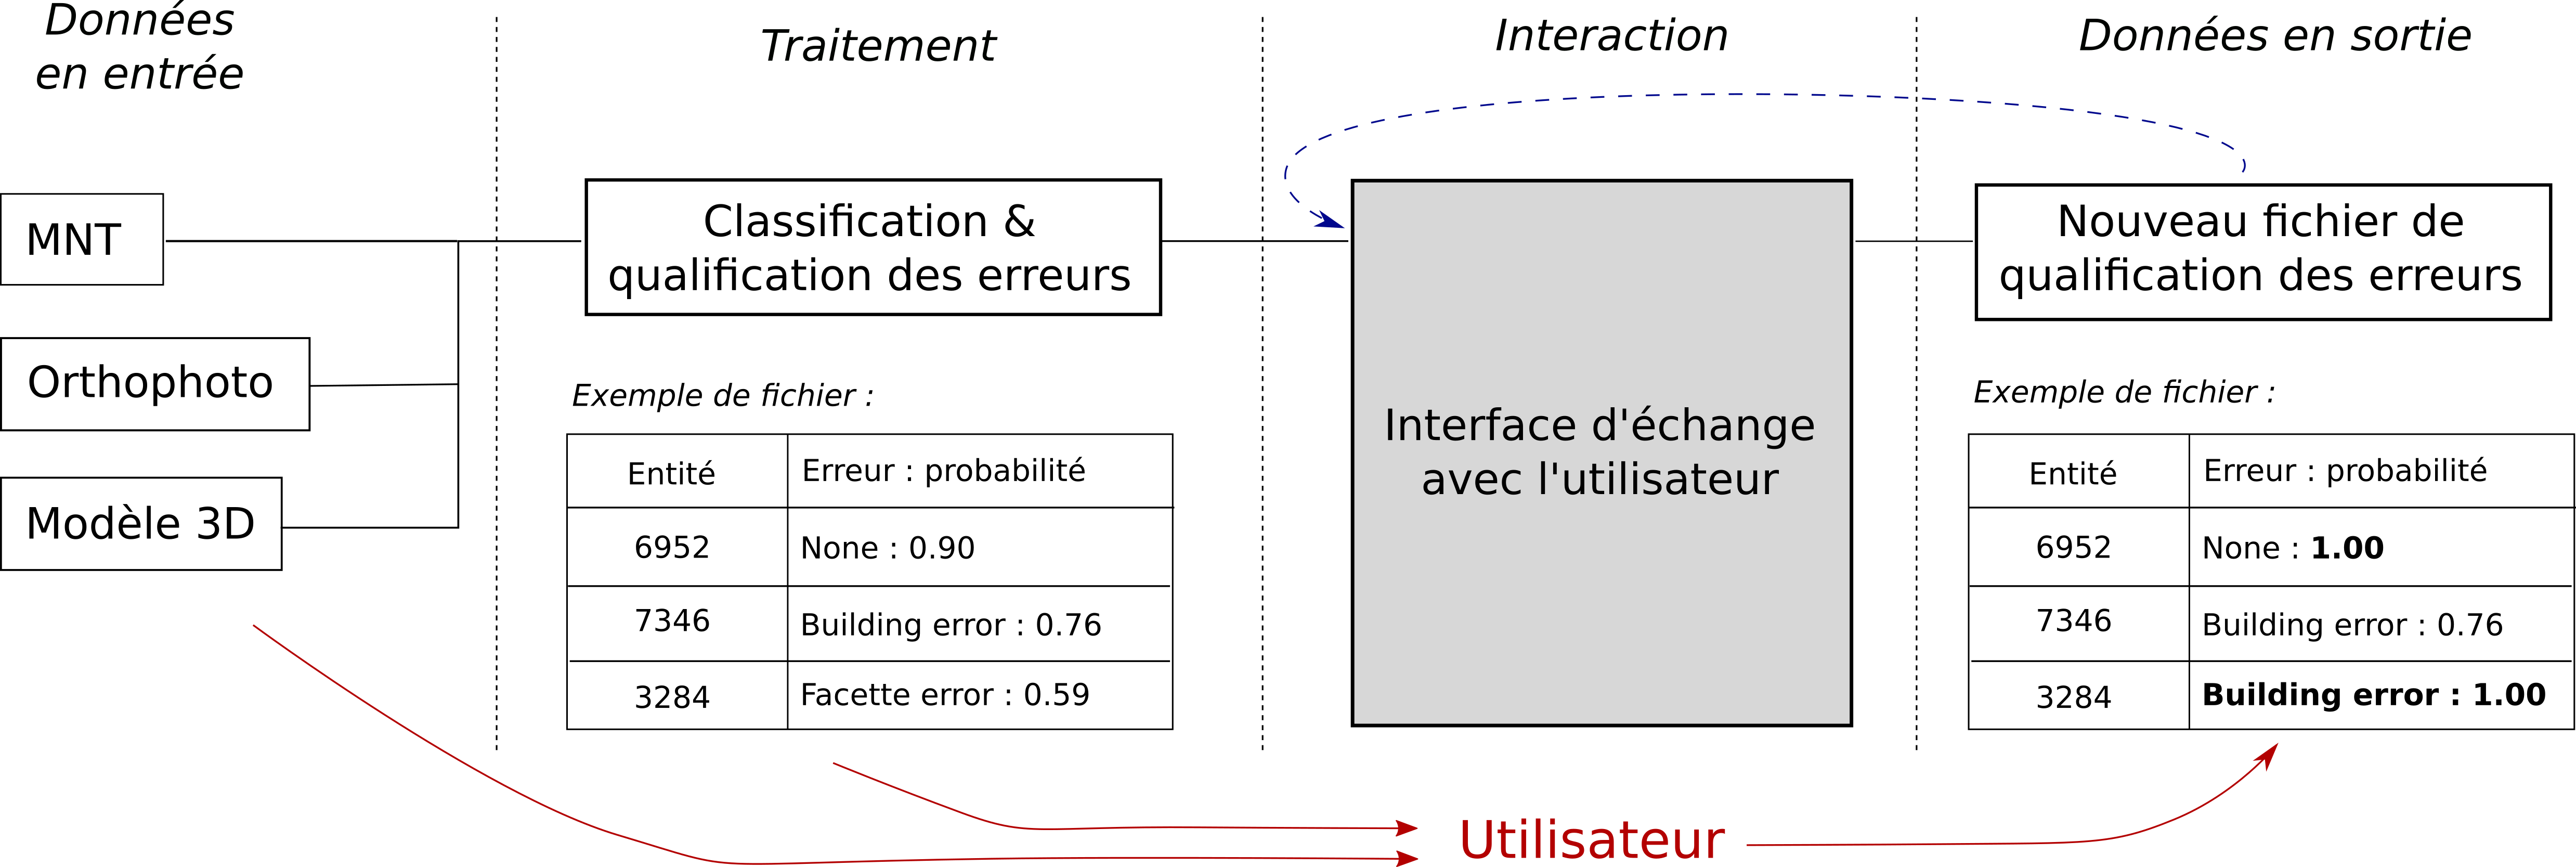
\includegraphics[scale=0.35]{Process_projet.png}  \\
		\caption[Chaîne de traitement simplifiée du projet]{Chaîne de traitement simplifiée du projet}
		\label{fig:processprojet}
	\end{center}
\end{figure}

\textit{Cette section a permis de retracer les principaux objectifs du projet. Le développement suivant vise à détailler les principales fonctionnalités envisagées lors de l'analyse.}

\section{Analyse fonctionnelle}

\subsection{Organisation des données}

Le programme considère plusieurs données en entrée, sélectionnées par l'utilisateur via une première interface :

\renewcommand{\arraystretch}{1.4}
\begin{figure}[!h]
	\begin{center}
		\begin{tabular}{|c|c|c|}
			\hline
			Données & Type de donnés & Correspondance dans le code \\
			\hline
			Classes d'erreurs possibles & Fichier .CSV & Variable de type dictionnaire \\
			Résultats de l'auto-qualification & Fichier .CSV & Liste de tuples \\
			Géométrie des entités & Dossier de .SHP & Attribut \textit{geometry} de la classe Bâtiment\\
			Orthophoto & Fichier .TIFF & Tuple (résolution + référence) + Matrice\\
			\hline
		\end{tabular}
	\end{center}
	\caption[Données en entrée]{Données en entrée}
	\label{tab:dataentre}
\end{figure}

\noindent De même, le formalisme des données en sortie est imposé :

\renewcommand{\arraystretch}{1.4}
\begin{figure}[!h]
	\begin{center}
		\begin{tabular}{|c|c|c|}
			\hline
			Données & Type de donnés & Correspondance dans le code \\
			\hline
			Résultats de l'interaction & Fichier .CSV & Liste de tuples \\
			\hline
		\end{tabular}
	\end{center}
	\caption[Données en sortie]{Données en sortie}
	\label{tab:datasortie}
\end{figure}

\subsection{Principales fonctionnalités}

\begin{figure}[!h]
	\begin{minipage}{0.50\linewidth}\parindent12pt
		 \indent L'interface doit permettre à un utilisateur de visualiser et de contrôler les résultats d'une classification. Ainsi, les principales fonctionnalités à développer sont :\\
		\begin{itemize}[label=$\rightarrow$]
			\item Une interface de chargement des données ;
			\item Une fonction de sélection des entités à présenter à l'utilisateur ;
			\item Une interface de visualisation graphique et textuelle des entités ;
			\item Une fonction de contrôle des entités par l'utilisateur.
		\end{itemize}
	\end{minipage}
\hfill
	\begin{minipage}{0.45\linewidth}
		\centering
		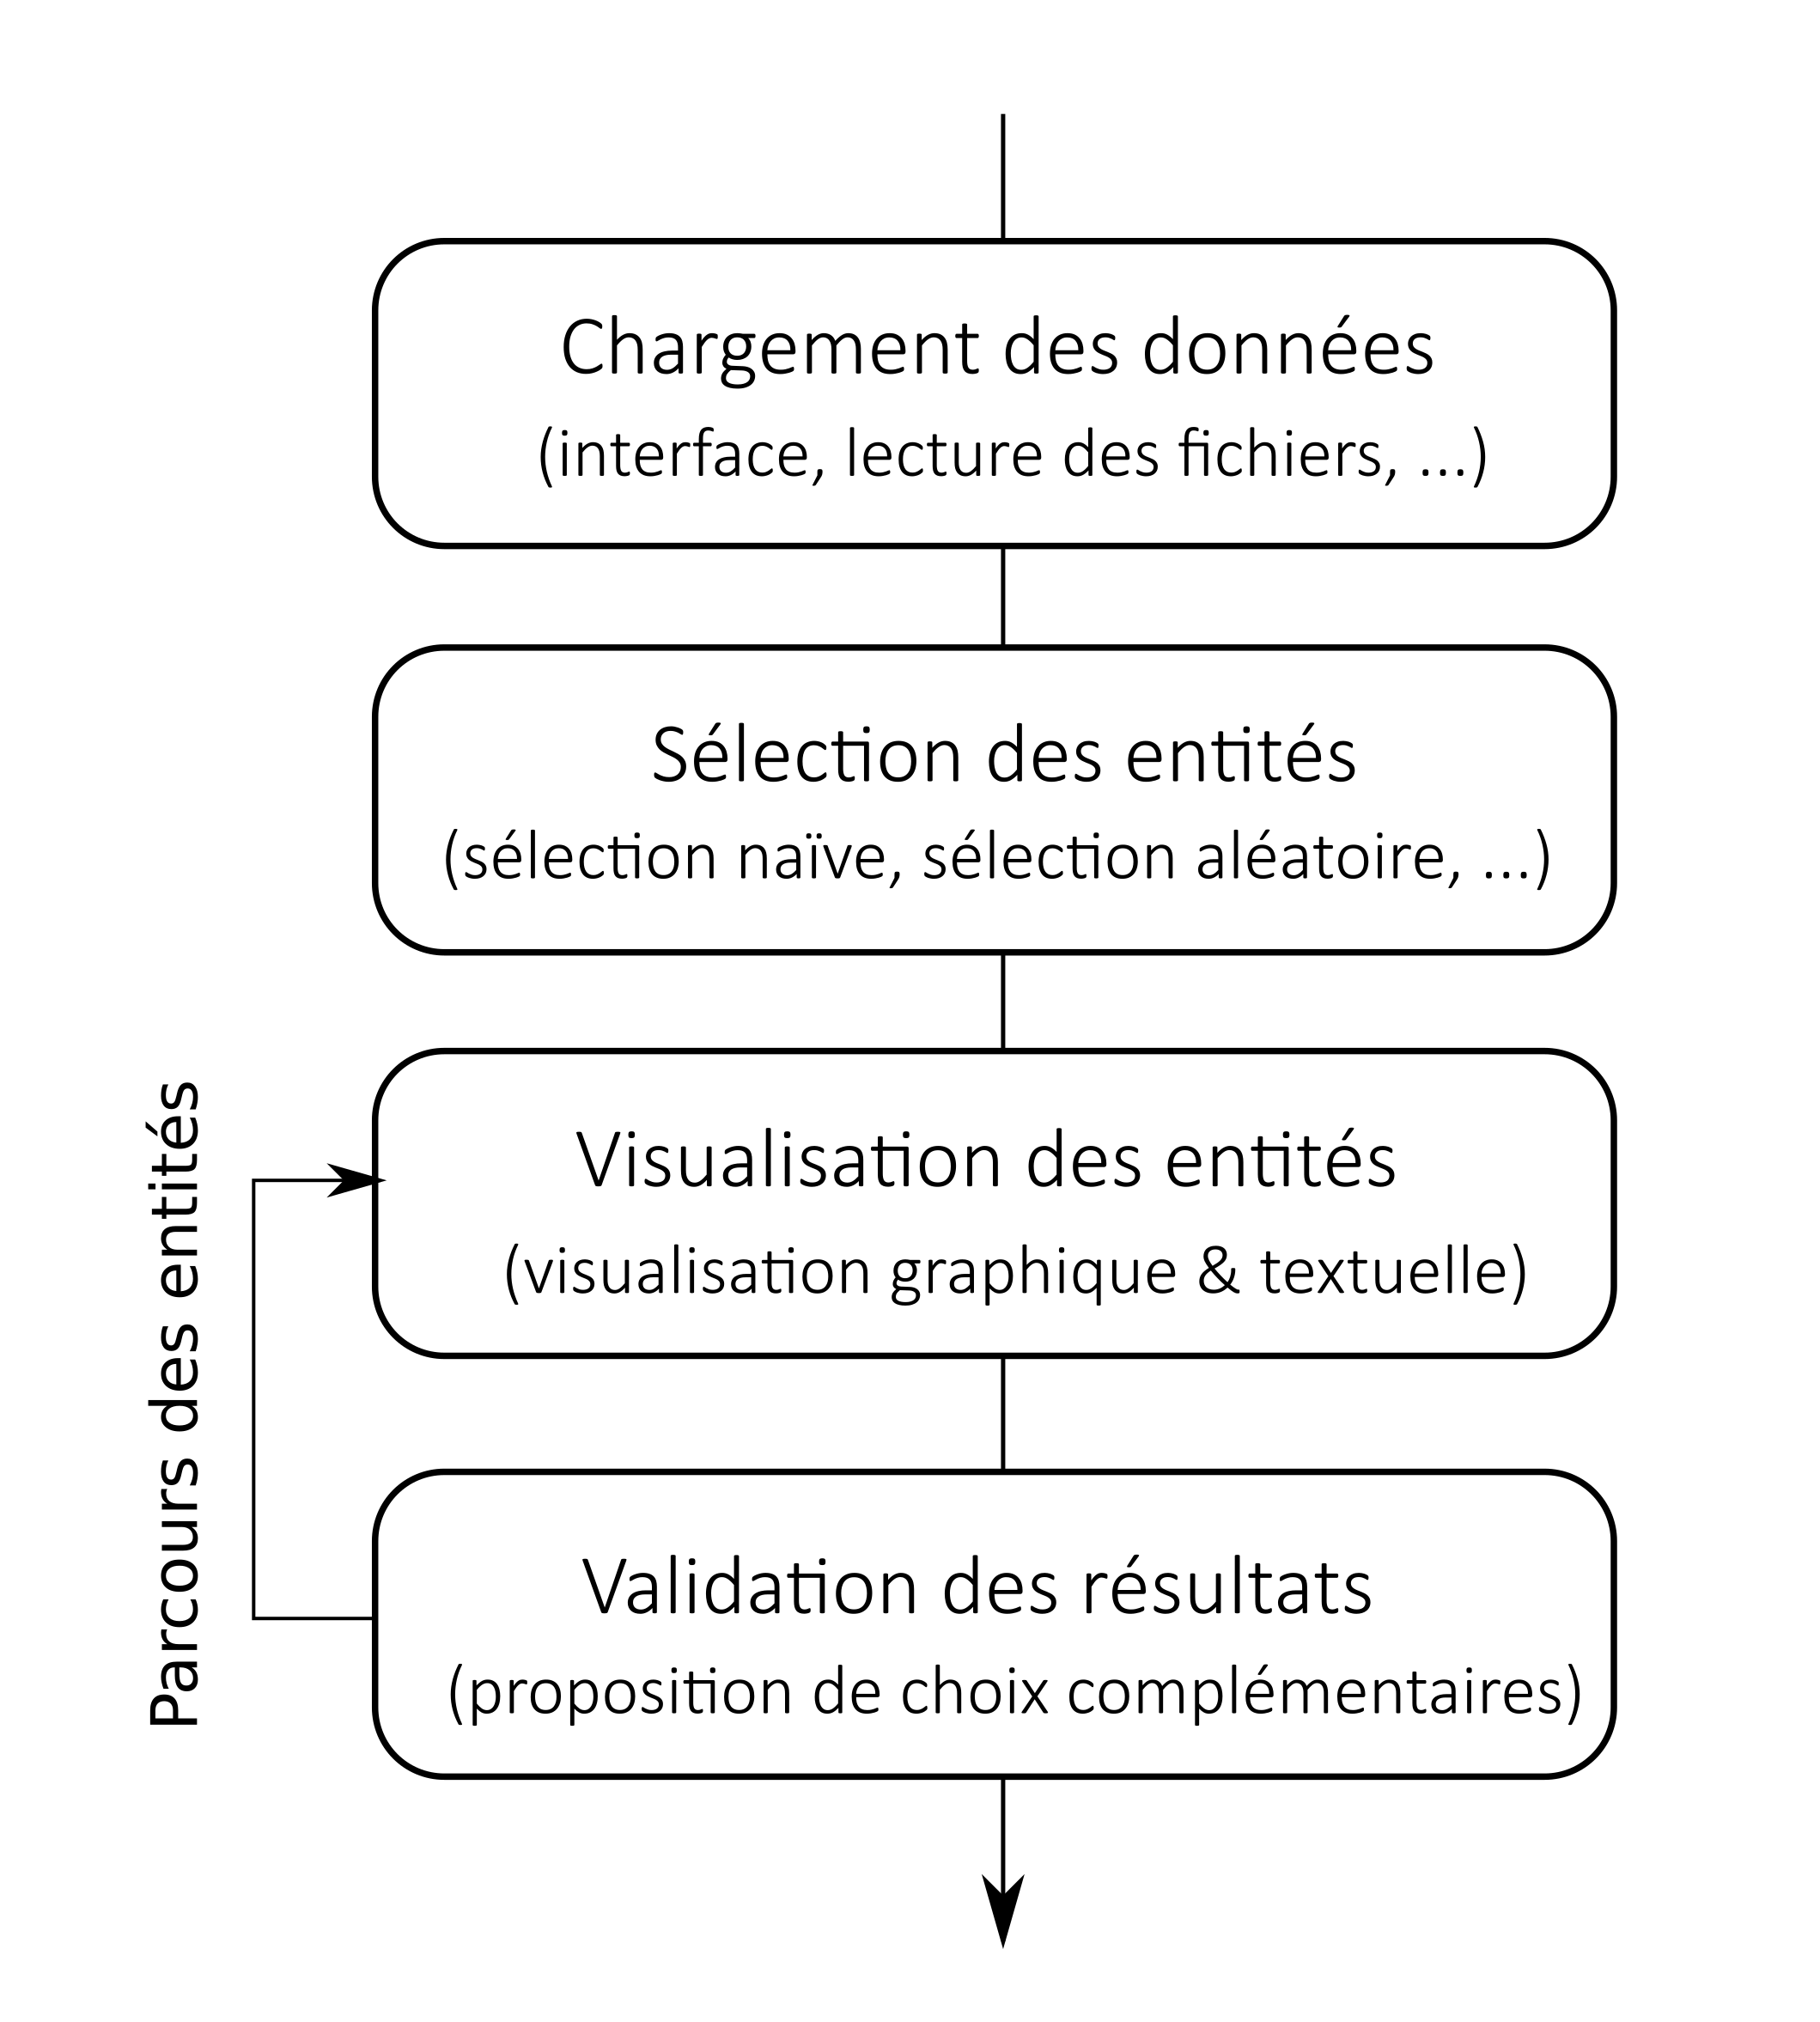
\includegraphics[scale=0.30]{Fonctionnalites_principales.png}  \\
		\caption[Fonctionnalités principales]{Fonctionnalités principales}
		\label{fig:fonctionnalitesprinc}
	\end{minipage}
\end{figure}

\textit{Après avoir rappelé les principales fonctionnalités du programme et les données nécessaires à son fonctionnement, on rappellera les choix techniques réalisés.}

\section{Choix techniques}

L’interface graphique voulue pour ce projet utilise la bibliothèque Qt associée à un programme Python (PyQt5). C'est une solution indépendante et multiplateforme. Elle peut être exécutée sur tous les environnements, et elle ne dépend pas de l'évolution d'un autre framework, par exemple QGIS.
\chapter[Détail du code]{Détail du code}

\textit{Pour faciliter l'écriture et la compréhension du code, on utilise la méthode Modèle/Vue/Contrôleur. Dans cette section, on détaillera donc les différentes fonctions implémentées en suivant ce modèle.}

\section{Partie Vue}

La partie Vue contient le code relatif à l'interface graphique. Après la réalisation des trois interfaces graphiques avec QtDesigner, l'utilitaire PyUic5 a permis de transcrire le code C++ en langage Python. \\

\noindent Trois fichiers ont alors été créés et définissent les trois classes :
\begin{itemize}[label=$\rightarrow$]
	\item La classe \textit{Ui\_InterfacePrincipale} du fichier \textit{classificationActive.py} comporte le code de l'interface principale. Elle définit les caractéristiques des boutons, des labels de texte et de la fenêtre graphique dans une première méthode \textit{setupui} : ce sont les attributs de l'interface. Une méthode \textit{retranslateUi} permet de mettre à jour le texte des attributs.\\
	\item La classe \textit{Ui\_ChargementFichiers} du fichier \textit{chargementFichiers.py} comporte le code de l'interface de chargement. Elle dispose elle aussi des deux méthodes \textit{setupui} et \textit{retranslateUi}. Pour permettre l'affichage des différentes stratégies dans le menu déroulant, on utilise la variable globale STRATEGIES définie dans le fichier \textit{strategy.py}. Ainsi, ce menu sera mis à jours automatiquement en cas d'implémentation d'une nouvelle stratégie.\\
	\item La classe \textit{Ui\_ChoixClasse} du fichier \textit{choixClasse.py} comporte le code de l'interface de sélection d'une nouvelle classe. Elle dispose des méthodes \textit{setupui} et \textit{retranslateUi}.\\
\end{itemize}

En cas de modification de l'interface, ces fichiers sont réécrits, mais cela n'impactera pas le code du programme principal. Une seule modification doit être apportée à ces codes générés automatiquement : il faut modifier le chemin de l'image du point d'interrogation. En effet, ce chemin est contenue dans un fichier ressource en C++, qui n'est pas traduisible simplement en Python avec PyUic5. 

\section{Partie Modèle}

La partie Modèle contient organise le formalisme des données. Ainsi, trois nouveaux fichiers viennent définit trois classes : la classe \textit{Building}, la classe \textit{Background} et la classe \textit{Strategy}.\\

\subsection{La classe \textit{Building}}

La classe \textit{Building} est codée dans le fichier \textit{building.py}. Un objet de type \textit{Building} est défini par 4 attributs : identity (identifiant de l'objet), geometry, classe et probability. Deux méthodes lui sont associées : 
\begin{itemize}
	\item \textit{get\_points} retourne la liste de tous les sommets de chaque géométrie de l'entité. Ainsi, si une entité est composée de 3 triangles, la liste de sortie contiendra 9 points. Chaque point est codé par un couple de coordonnées (x,y).
	\item \textit{get\_bounding\_box} parcourt l'ensemble des coordonnées x et y d'une liste et retourne les valeurs maximales et minimales de ces deux paramètres. Cela permet de définir la fenêtre d'emprise d'une entité.
\end{itemize}


\section{Partie Contrôleur}
\chapter[Limites et évolutions de la solution]{Limites et évolutions de la solution}

\textit{La phase de programmation a permis de développer une première solution au sujet posé. Cependant, certaines fonctionnalités manquent encore. Ce chapitre détaille donc les améliorations pouvant être apportées au programme.}

\section{Limites de la solution proposée}

Bien que la solution proposée soit fonctionnelle et réponde à la problématique du projet, certaines fonctionnalités manquent encore :
\begin{itemize}[label=$\rightarrow$]
	\item Fonction de zoom : pour permettre à l'utilisateur d'agrandir ou de réduire l'entité présentée, une fonction de zoom peut être implémentée. Cette fonctionnalité pourra se baser sur les méthodes de la classe \textit{QGraphicsView}, et sur une fonction enregistrant les rotations de la molette de la souris.
	\item Gestion des marges trop grandes : dans la fenêtre de chargement, l'utilisateur peut définir des marges pour visualiser l'environnement des bâtiments. Pour l'instant, aucune fonctionnalité ne gère les cas de marges dépassant les bordures de l'orthoimage.
	\item Affichage des MNS : grâce aux méthodes de la classe \textit{QPixMap}, l'interface peut afficher une orthoimage couleur, constituée de trois bandes. Une nouvelle fonctionnalité pourrait gérer le cas de l'afficher des MNS constitués d'une seule bande. \\
\end{itemize}

De plus, l'implémentation de cette solution a été réalisée en s'appuyant sur un jeu de données types. Leur formalisme étant imposé à l'utilisateur, le programme devrait fonctionner avec d'autres données. Cependant, des tests complémentaires pourraient être réalisés pour vérifier la compatibilité de l'interface (utilisation d'une autre orthophoto, utilisation de plus d'emprises, ...).


\section{Évolution de la solution}

- Autres méthodes de filtrage\\
- Autre type de classification\\



%\begin{comment}
%-------------------------------------------------------------------------------
\newevenpage
\chapter*{Conclusion}
  \addcontentsline{toc}{part}{Conclusion}
  \vspace{1.5cm}
Il est l'heure de conclure : bonne nuit !


%-------------------------------------------------------------------------------
% Insertion de la bibliographie
\newevenpage
\printbibheading
\printbibliography[title={Bibliographie}]
\nocite{*}

\newevenpage
\listoffigures

\newevenpage
\listoftables
%----------------------------------------------------

\newevenpage
\begin{appendices} 
\label{beginappendices}
\annexe[Filtre de Kalman]{Filtre\newline de Kalman}
\label{annexekalman}
Annexe 1

\end{appendices} 
%\end{comment}
\end{document}